\section{Multi-criteria decision analysis for process selection}

Chemical process development and especially synthesis route selection are regarded as the most critical conceptual design step since those major decisions affect the whole process lifecycle \cite{cziner_evaluative_2005}. Locating one optimum solution from several non-dominating plausible alternatives is challenging due to the necessity of considering various, and often conflicting, criteria. To help stakeholders make systematic and informed decisions for key aspects of the process, multi-criteria decision making (MCDM) methods have been developed. Those tools provide a quantitative and comparative evaluation of alternatives meeting design requirements, thus minimising subjectivity and bias \cite{greco_multiple_2016}. 
This section discusses Nitroma's selection procedure for the three products to be produced in its multi-purpose plant, and their associated synthesis routes. Employing both a qualitative approach and MCDM methods, greater importance was given to safety and environmental concerns, technical performance and economic potential of different options.

\nomenclature[A]{MCDM}{Multi-criteria decision making}

\subsection{Selection of MCDM} %~0.5 page

Numerous computer-based MCDM methods have been developed over the last few decades to respond to the need for systematic decision making tools. Based on different theories and assumptions, those methods have unique characteristics which render them more suited for certain areas of application. Several well-known MCDM methods were initially considered, including multi-attribute methods: Weighted Sum method (WSM), Multi-Attribute Utility Theory (MAUT) and Analytic Hierarchy Process (AHP); and outranking methods: Elimination and Choice Expressing Reality (ELECTRE),  Technique for the Order Preference by Similarity to Ideal Solution (TOPSIS) and Preference ranking organization method for enrichment evaluation (PROMETHEE) \cite{hodgett_multi-criteria_2013}. 

Due to inherent limitations of all methods, a combination of at least two methods will be used to ensure a more accurate decision is made \cite{greco_multiple_2016}. AHP and TOPSIS were found to be the most suited methods after consideration of the advantages and disadvantages of each technique. Despite its straightforward application, WSM is not capable of handling multi-dimensional decision-making problems, thus leading to results always not reflecting the real situation \cite{pohekar_application_2004}. AHP provides an easy to use and scalable hierarchical structure which can accommodate multiple options and criteria, but which is not as data intensive as MAUT \cite{velasquez_analysis_2013}. Moreover, as opposed to MAUT which requires very precise input data, AHP can handle problems with  non-monetary criteria when limited information can be found in literature \cite{great_britain_multi-criteria_2009}. ELECTRE was eliminated due to its inapplicability to criteria with different ranges \cite{greco_multiple_2016}. In addition to the difficulties in strength and weakness identification for alternatives, PROMETHEE does not provide a clear procedure to assign weights to criteria \cite{velasquez_analysis_2013}. On the other hand, TOPSIS presents a simple process which is easy to use and program \cite{velasquez_analysis_2013}. Nonetheless, AHP and TOPSIS have limitations which can be overcome by combining the two methods, as discussed in the following section.

\nomenclature[A]{WSM}{Weighted Sum method}
\nomenclature[A]{MAUT}{Multi-Attribute Utility Theory}
\nomenclature[A]{AHP}{Analytic Hierarchy Process}
\nomenclature[A]{ELECTRE}{Elimination and Choice Expressing Reality}
\nomenclature[A]{PROMETHEE}{Preference ranking organization method for enrichment evaluation }
\nomenclature[A]{TOPSIS}{Technique for Order of Preference by Similarity to Ideal Solution}

\subsection{Combined AHP and TOPSIS analysis} %~0.5 page

The decision-making process using MCDM methods follows six steps \cite{great_britain_multi-criteria_2009}: (1) identify the options to be appraised, (2) identify criteria to asses the performance of each option, (3) scoring each option against a criteria, (4) assign criteria weightings, (5) compute, analyse and compare the weighted scores of each options, and (6) perform sensitivity analysis to evaluate the robustness of the final decision.
Process alternatives were initially short-listed with qualitative arguments (step 1) and then ranked with the quantitative processing of all relevant information against selection criteria (step 2) through AHP and TOPSIS analyses (step 5). 

AHP decomposes complex problems into structure hierarchies to find a unique optimum solution meeting the overall objective \cite{mu_practical_2017}. The analysis focus is broken down in categories made of several criteria which can be quantified with information available in literature. The categories and the criteria are independently compared pairwise using a 1-9 scale to assess the relative signification of one category/criteria over another \cite{saaty_analytic_1987}. Following the procurement of a set of category and criterion weights with pairwise comparison, the performance of each alternative is computed and a final ranking of solutions is obtained. The option with the highest sum of normalised scores is recommended. Several flaws of AHP have been identified, notably the ‘rank reversal’ phenomenon which occurs when the introduction of new options changes the relative ranking of some of the original options \cite{great_britain_multi-criteria_2009}. Moreover uncertainty is not directly accounted for and significant bias is introduced due to human judgement for the pairwise comparison \cite{millet_modelling_2002}. Those drawbacks can be addressed with built-in consistency checks of criteria weightings and combination with TOPSIS for quantitative reinforcement \cite{tzeng_multi-criteria_2005}. Nevertheless, AHP can produce solid weight estimation for categories which can then be fed into TOPSIS. 

On the contrary, criteria weightings and the associated inconsistency index can not be derived with TOPSIS alone \cite{roszkowska_multi-criteria_2011}. The basis concept of the TOPSIS method is that the best alternative is the one which has the shortest distance to the ideal solution and longest distance to negative ideal solution \cite{pohekar_application_2004}. The positive and negative ideal solutions are computed by respectively combining the best and worst performances for each criteria \cite{olson_comparison_2004}. It is assumed that each criteria varies monotonically. The decision matrix of M alternatives and N criteria is normalised and the alternatives are ranked through comparing the Euclidean distances to the ideal best and worst solutions. This method allow for trade-off between criteria and distinguish between criteria that needed to be maximised and ones that needed to be minimised \cite{pirdashti_multi-criteria_2009}. TOPSIS evaluation with criteria weightings derived from AHP is thus a suitable MDCM method for selecting the optimum products and synthesis routes.


\subsection{Sensitivity} %~0.5 page

Significant bias is introduced when deriving criteria weightings in AHP. The decision makers indeed subjectively determine the relative importance of one criteria over another \cite{triantaphyllou_sensitivity_1997}. Moreover, the nature of the selected judgement scale also influences the results and subsequent decisions \cite{franek_judgment_2014}. In this context, a sensitivity analysis of the effect of criteria weighting on the final scores for both AHP and TOPSIS was conducted. The criteria weightings were varied from 0 to 1 with 0.005 increments and a computational model was developed to perform the AHP and TOPSIS analysis for each of the weighting combination. This sensitivity analysis maps out in which range of criteria weightings would each alternative be optimum. The sensitivity analysis of scores was judged less relevant as all values inputted were based on physical data found through literature research.



\subsection{Products selection}

To deliver a multi-purpose plant, Nitroma selected toluene as feedstock due to the industrial importance of its nitration products and their amino derivatives. All three isomeric nitrotoluenes can indeed easily be oxidised and reduced to substituted aromatic amides of significant importance for the pharmaceutical, agrochemical and textile industries \cite{dugal_nitrobenzene_2005}. Six chemicals were initially selected due to their applications in drugs, fertilizers or dyes: 2-aminobenzaldehyde (precursor of quinoline derivatives for polymer, agrochemical, dye, antiviral and anti-malaria drug manufacturing), 4-aminobenzaldehyde (intermediate to pharmaceuticals and vanilin), 4-aminobenzoic acid (production of folic acid/vitamin B9), \ortho-toluidine (intermediate in the manufacture of herbicides), \meta-toluidine (manufacture of  photographic color developer) and \para-toluidine (for dye production) \cite{bowers_toluidines_2000,bruhne_benzaldehyde_2011,maki_benzoic_2000}. To determine the three most advantageous products to produce, AHP/TOPSIS analysis was conducted.

\subsubsection{Criteria identification and weighting}

The choice of criteria and the determination of their relative weightings have serious implications in the decision making process. In order to ensure long term business sustainability, aspects not limited to economic profitability were considered. Nitroma's product selection must indeed enable the development of a commercially feasible and inherently safe process for products where strong demand exists. As such, the analysis focused on three main categories: economic potential, process complexity and environment, health and safety (EHS) considerations. The social aspect was not included in the analysis since it is expected all products would have created similar employment opportunities in the plant. 
The economic potential of each chemical was determined using the average price, the average market share of current producers, the global demand for the products and the expected market growth (CAGR). The market share was valued twice as much as the other sub-criteria since it is an indicator of type of market of this industry and helps predict the market share Nitroma can plan to capture. For all the economic sub-criteria, a higher score is preferable. Process complexity refers to the number of reactions following nitration to reach the desired products, the lower the better. The maximum selectivity of nitration towards a product is an indicator of the nitrotoluene isomers rate which can be expected without modification of the selectivity via process conditions (catalyst, solvent, temperature). Safety was assessed using the NFPA Hazard Classification for health, flammability and instability, where the smallest value is preferable. Since there exist a several possible synthesis routes for each product, and that those were found to have a significant degree of similarity, the safety and environmental impacts of the reaction conditions were not evaluate at this point since it would not help in comparing different final products. 

Weightings for the three categories was done via the AHP methodology. \Cref{tab:pairwise} for pair-wise criteria comparison can be found in \Cref{app:matrix}. Significant importance was given to the safety of the compounds (57\%), reflecting Nitroma's commitment to develop an inherently safe process. Economic potential (29\%) was valued more importantly than process complexity (14\%) since the data used results for a preliminary study of reaction routs which will be later refined to maximise production of the selected products. The consistency ratio was calculated to ensure the criteria and their weightings are linearly independent. With a 3\% consistency ratio, the weightings are deemed consistent since they don't exceed the 10\% inconsistency threshold \cite{saaty_analytic_1987}.


\nomenclature[A]{NFPA}{National Fire Protection Association}
\nomenclature[A]{CAGR}{Compound annual growth rate}



\subsubsection{Results}
\Cref{tab:product} summarises the results from AHP and TOPSIS analysis.   
Due to their high economic potential and reduced health and fire hazards, 4-aminobenzaldehyde (4-ABH), o-toluidine (o-TOL), and 4-aminobenzoic acid (4-ABA) were found to be the most suitable products. This implies that Nitroma's process will simultaneously products \ortho and \para derivatives of nitrotoluenes. Plant modularity arises from the ability to switch between a 4-ABH focused and 4-AB1 focused production lines. A summary of the selected products and their associated synthesis pathways can be found in \Cref{fig:routes-chosen}.

\begin{table}[h]
\centering
    \caption{AHP/TOPSIS results for product selection}
    \label{tab:product}\footnotesize
\begin{tabularx}{\linewidth}{l|S[table-format=4.2]S[table-format=1.1]XS[table-format=7.0,round-mode=figures,round-precision=2]|XX|lll|S[table-format=1]S[table-format=1]c}
\toprule
                                          & \multicolumn{4}{c}{Economic potential   (\SI{29}{\percent})}                                & \multicolumn{2}{|>{\hsize=\dimexpr2\hsize+2\tabcolsep}X}{Process   complexity (\SI{14}{\percent})} & \multicolumn{3}{|c|}{EHS (\SI{57}{\percent})}     &                       &                          &                           \\ \cmidrule{2-10}
                                          & {\splitcell{Price\\(\si{\USD\per\kg})}} & {\splitcell{CAGR\\(\%)}} & \rcell{Average market share of producer (\%)} & {\splitcell{Demand\\(\si{\tonne\per\year})}} & \rcell{Number of reactions} & \rcell{Max selectivity to toluene (\%)} & \rtext{Health} & \rtext{Flammability} & \rtext{Instability} & AHP & TOPSIS & Rank \\ \midrule
2-aminobenzaldehyde & 133.10          & 5.6 & 0.77                           & 1300                 & 2                & 53                       & 2      & 1            & 1           & 0.124                 & 0.273                    & 6                         \\ 
4-aminobenzaldehyde & 19.00            & 7.1 & 1.75                           & 34000               & 2                 & 44                       & 2      & 1            & 0           & 0.188                 & 0.563                    & \cellcolor{green}2 \\ 
o-toluidine         & 10.62           & 7.8 & 0.88                           & 810000              & 1                   & 53                       & 3      & 2            & 0           & 0.210                 & 0.611                    & \cellcolor{green}1 \\ 
p-toluidine         & 9.00             & 6.3 & 0.50                           & 60000               & 1                   & 44                       & 3      & 2            & 0           & 0.150                 & 0.333                    & 5                         \\ 
m-toluidine         & 8.90           & 8.2 & 0.57                           & 110000              & 1                   & 3                       & 4      & 2            & 0           & 0.161                 & 0.458                    & 4                         \\ 
4-aminobenzoic acid & 26.29         & 5.8 & 3.70                           & 3250               & 2                 & 44                       & 2      & 1            & 1           & 0.168                 & 0.478                    & \cellcolor{green}3 \\ \bottomrule
\end{tabularx}
\end{table}




\nomenclature[A]{4-ABH}{4-aminobenzaldehyde}
\nomenclature[A]{o-TOL}{o-toluidine}
\nomenclature[A]{4-ABA}{4-aminobenzoic acid}

\subsubsection{Sensitivity}

The weightings of the three criteria were varied from 0 to 1 simultaneously to map out the range of validity for each combination of products. It was found that 7 combinations of three products could be optimum depending on the relative importance given to each criteria. \Cref{fig:sensitivity_product} shows for which criteria weightings each combination was returned by AHP and TOPSIS analysis as optimum. Nitroma's selected combination of product, in red, is located in the centre of the ternary diagrams, indicating that it represents a good compromise between all criteria with moderate relative importance. The combination excluding toluidine isomers (in dark blue) is optimum when safety and environmental considerations are highly valued compared to the economic potential, reflecting the more benign nature for aminobenzaldehydes and amino benzoic acid. 

\begin{figure}[h]
    \centering
    \subfloat[AHP]{{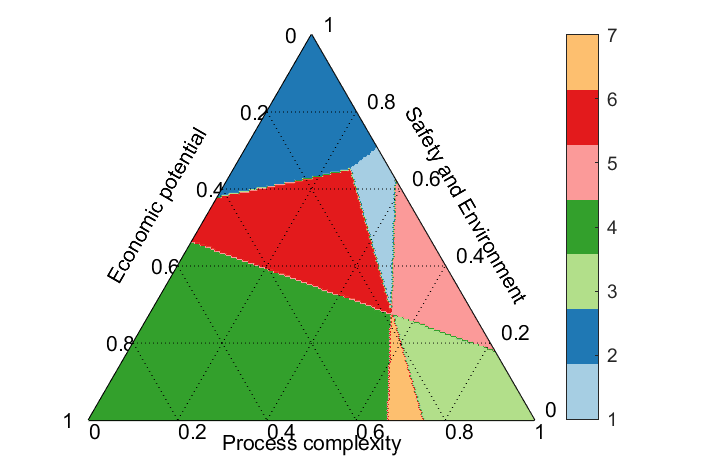
\includegraphics[width=.46\linewidth]{chapters/1-synthesis/1-Figures/AHP_product.pdf} }}
    \qquad
    \subfloat[TOPSIS]{{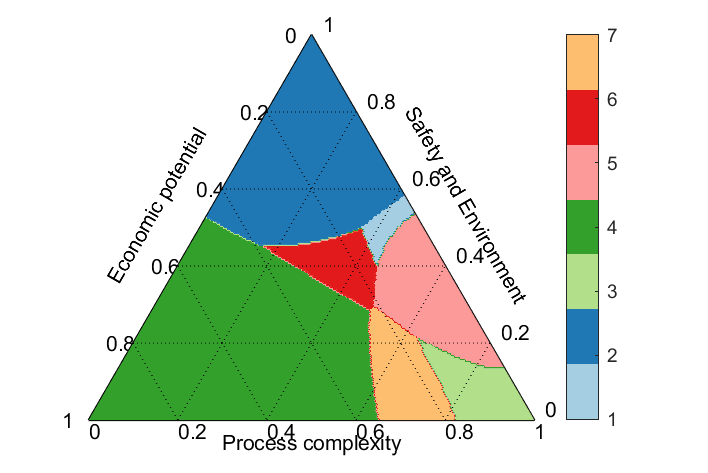
\includegraphics[width=.46\linewidth]{chapters/1-synthesis/1-Figures/TOPSIS_product.pdf} }}
    \caption{Sensitivity analysis of AHP and TOPSIS results for product selection. Legend: (1) 2-ABH, 4-ABH, o-TOL; (2) 2-ABH, 4-ABH, 4-ABA; (3) 2-ABH, o-TOL, p-TOL; (4) 2-ABH, o-TOL, 4-ABA; (5) 4-ABH, o-TOL, p-TOL; (6) 4-ABH, o-TOL, 4-ABA; (7) o-TOL, p-TOL, 4-ABA}%
    \label{fig:sensitivity_product}%
\end{figure}

\subsection{Nitration reaction}

Nitration is a highly exothermic reaction between a nitration agent and an organic compound, resulting in the chemical bonding of a nitro group (\ch{NO2}) to an atom in this compound. Nitration of aromatics involves the use of a strong acid to catalyse the formation of nitronium ions \ch{NO2+}. This section will review the selection of nitrating agent and catalyst, as well as Nitroma's strategy to mitigate nitrogen oxide emissions associated with nitration.

\subsubsection{Choice of nitrating agent}

Nitric acid has been selected as the source of nitrogen for the nitration of toluene for its safe and environmentally friendly nature relative to other possible nitrating agents and its high availability \cite{miller_kinetics_1964, sreedhar_scientific_2013}. Although nitric acid is a highly acidic and volatile compound, compared to alternatives such as acetone cyanohydrin and dinitrogen tetroxide which are highly toxic, nitric acid is more appropriate for industrial-scale nitration of toluene \cite{dagade_nitration_2002, sreedhar_scientific_2013}. Nitric acid, introduced as an aqueous solution, is the most commonly used and well-studied nitrating agent for this process in industry. \cite{bowers_toluidines_2000}. A common alternative to nitric acid is acetyl nitrate which is formed by the reaction of nitric acid with acetic anhydride \cite{vassena_selective_1999}. This reaction however yields formic acid, acetyl nitrate and acetic anhydride as by-product, resulting in a lower atom economy and additional difficulties in separations downstream. The same argument can be employed for other alkyl nitrates such as butyl nitrate. To this end, nitric acid is deemed as the most suitable choice among all candidates.

\subsubsection{Choice of catalyst}

Commercial production of nitrotoluene is mainly carried out by a mixed-acid process, whereby sulfuric acid donates a proton to nitric acid, yielding a nitronium ion which will then react with toluene \cite{halder_nitration_2007}. In a continuous adiabatic process, toluene and nitric acid are fed into a large recycle stream of sulfuric acid. The composition of the mixed-acid is typically \SI{20}{\percent} \ch{HNO3}, \SI{60}{\percent} \ch{H2SO4} and \SI{20}{\percent} \ch{H2O} \cite{pande_nitration_2010}. Toluene is in excess of \SI{10}{mol\percent} with respect to nitric acid to completely consume nitric acid, thus avoiding avoid the formation of dinitrotoluene. The reaction takes place in a PFR with static mixers or a cascade of CSTR \cite{dugal_nitrobenzene_2005}. The organic phase is separated in a decantor while the sulfuric acid is regenerated in a reconcentration step. Yields up to \SI{96}{\percent} can be obtain with this process. However the 0.6 \textit{para}/\textit{ortho} ratio is commercially unfavourable. In addition to favouring less economically desirable \textit{ortho} isomers, more complex product separation and acid regeneration are expensive and energy intensive \cite{sreedhar_scientific_2013}. Moreover, the high E-factor of the reaction, resulting from the large amount of 'spent acid', attests of the environmentally unfriendly nature of this process catalysted by hazardeous and corrosive sulfuric acid \cite{pande_nitration_2010}. These drawbacks can be overcome by solid acid catalysts which offer an environmentally friendly and economic alternative to mixed-acid processes \cite{vassena_selective_1999}.

 Based on those arguments, Nitroma will develop a safer and low environmental impact process employing zeolite catalysts for toluene nitration. More specifically, the relative benefits and disadvantages of 3 different zeolites were evaluated with the AHP and TOPSIS decision analysis methods to select the optimum catalyst. The economic potential, performance and safety of zeolites H-ZSM-5, H-Y and H-Mordenite were assessed and compared to the case with no catalyst \cite{jeeru_kinetics_2018}.  The economic potential was measured with the cost of the catalyst and the percentage of undesirable dinitrotoluene by-product formed. Conversion and the NFPA score are the KPIs for performance and safety respectively. The scores and criteria weightings are displayed in \Cref{tab:nitration}. Catalyst performance was deemed priority by the decision makers since the cost of the different catalysts are fairy similar and that their EHS impact is comparable. Based on those weightings, H-Mordenite was found optimum for the catalytic nitration of toluene by both AHP and TOPSIS analysis, mostly due to the achieved high conversion rates. An additional benefit of H-Mordenite is its high reusability rate. Following three recycling cycles, the catalytic activity of the zeolite was found to have only marginally decreased \cite{jeeru_kinetics_2018}. 


\begin{table}[h]
\centering
    \caption{AHP/TOPSIS results for Nitration Catalyst Selection}
    \label{tab:nitration}\footnotesize
\begin{tabular}{l|S[table-format=2.3]S[table-format=1.2]|S[table-format=2.0]|lll|S[table-format=1.3]S[table-format=1.3]c}
\toprule
                                          & \multicolumn{2}{c|}{Economic potential   (\SI{14}{\percent})}                                & {Performance (\SI{57}{\percent})} & \multicolumn{3}{c|}{EHS (\SI{29}{\percent})}     &                       &                          &                           \\ \cmidrule{2-7}
                                          & {\splitcell{Price\\(\si{\EUR\per\g})}} & {\splitcell{By-products\\(\%)}} & {Conversion (\%)}  & \rotatebox[origin=r]{90}{Health} & \rotatebox[origin=r]{90}{Flammability} & \rotatebox[origin=r]{90}{Instability} & AHP & TOPSIS & Rank \\ \midrule
H-ZSM-5 & 0.734        & 0.5 & 41                             & 2       &  0          &     0       & 0.297                 & 0.752                & 2                         \\ 
H-Y & 0.696            & 0.48 & 36                           & 2      &        0     & 0           & 0.276                 & 0.705                   & 3 \\ 
H-Mordenite       & 0.726           & 0.55  & 43                            & 2      &     0        & 0           & 0.303                 & 0.761                  & \cellcolor{green}1 \\ 
No catalyst         & 0            & 0 & 2                         & 0      & 0            & 0           & 0.124                 & 0.237                    & 4                         \\ 
\bottomrule
\end{tabular}
\end{table}

Sensitivity analysis of the criteria weightings was then carried out to ensure the robustness of the decision. \Cref{fig:catalyst} shows the weighting ranges where each alternative is found optimum by AHP and TOPSIS analysis. H-Mordenite (light green) is favoured for high importance in process performance. It is is good compromise between technological interests and economical and EHS considerations. No catalyst is a suitable option when safety is the main concern, however the very low conversion makes this process not technical and commercially viable. Overall, there is a good concordance between the results from both MCDM methods, thus supporting Nitroma's selection of H-Mordenite catalyst.

\begin{figure}[h]
    \centering
    \subfloat[AHP]{{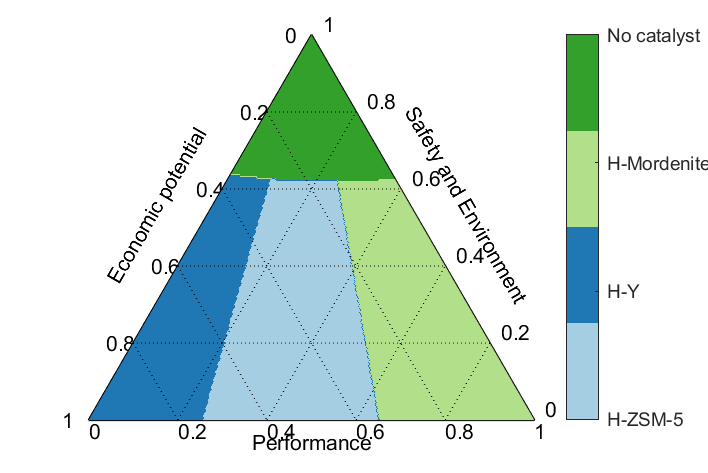
\includegraphics[width=.46\linewidth]{chapters/1-synthesis/1-Figures/AHP_nitration.pdf} }}
    \qquad
    \subfloat[TOPSIS]{{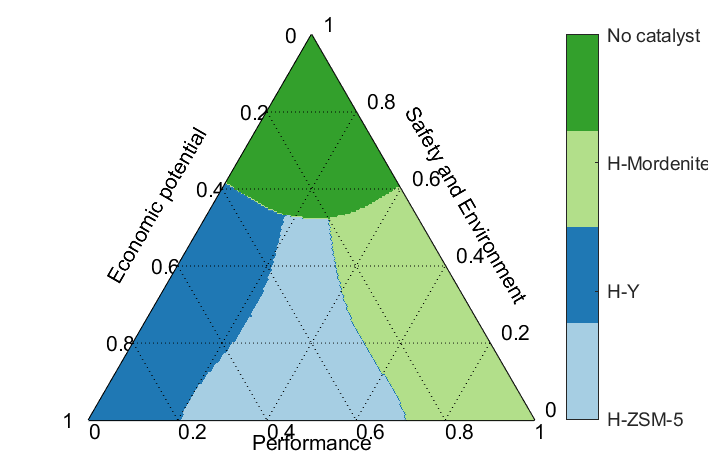
\includegraphics[width=.46\linewidth]{chapters/1-synthesis/1-Figures/TOPSIS_nitration.pdf} }}
    \caption{Sensitivity analysis of AHP and TOPSIS results for nitration catalyst selection.}%
    \label{fig:catalyst}%
\end{figure}

\subsubsection{NOx emission mitigation}

Nitrogen oxides are poisonous and highly reactive compounds which often appear as brownish gas. NOx can react with chemicals in the atmosphere, mailny water and oxygen to form acid rain which causes forest decline and fish mortality in sensitive ecosystems []. Due to its oxidative nature, NOx also plays a major role in photochemical ozone creation, resulting in smog on hot summer days []. Additionally, nitrogen oxides are known to have adverse effects on  health, causing respiratory conditions and  inflammation of the airways []. 

Emissions of NOx during nitration has been widely reported for mixed-acid processes\cite{halder_nitration_2007,processes_research_inc_air_1972}. \ch{HNO3} in sulfuric acid solutions is indeed known to decompose at high temperature to nitrogen oxides via a mechanism involving \ch{N2O5} \cite{robertson_kinetics_1955, kazakov_kinetics_1987}. However, to the best of our knowledge, no evidence of NOx emissions for processes with zeolite catalysts have been reported in literature \cite{vassena_selective_1999,sreedhar_scientific_2013}. The hypothesis for this observation is that the NOx formed from nitric acid decomposition is quickly reacted with zeolites to participate as a nitrating agent for toluene nitration \cite{akolekar_high_1995}. \textcite{akolekar_high_1995} indeed proposed a reaction mechanism whereby \ch{NO2} is at equilibrium with \ch{N2O4}, which then reacts with the protons from the zeolites to give \ch{NO+} and nitric acid. While the reformed nitric acid nitrates toluene with the help of the solid acid catalyst, \ch{NO+} bonds with aromatic ring and is later substituted by \ch{NO2}. Since the \ch{NO2}/\ch{N2O4} equilibrium leans towards \ch{N2O4}, we can assume that this reaction mechanism is very fast, thus comforting the experimental observations \cite{university_of_texas_chapter_nodate}. Furthermore, recent research on toluene nitration with NOx as nitrating agent over zeolites has been carried out. Publications have reported \SI{100}{\percent} and \SI{90}{\percent} toluene conversion with respectievly H-Beta and H-ZSM-5 zeolites \cite{pande_nitration_2010, peng_zeolite-assisted_2001}.

Owing to the decision of using a solid acid catalyst instead of sulfuric acid, Nitroma's process will not be emitting polluting and hazardous nitrogen oxides. However for completeness, the nitration reactor will feature a gas vent and a worst case scenario will be developed with a typical emission factor for mixed-acid processes to examine the potential problems from an environmental point of view.

\subsection{o-toluidine production}

Catalytic hydrogenation is the most efficient process for the large-scale reduction of nitrocompounds to their aromatic amines []. In the Béchamp process, the oldest commercial process for preparing amines, reduction takes place in the presence of iron and hydrochloric acid []. This process has now widely been replaced by continuous high pressure catalytic hydrogenation in the vapour or liquid phase, either with or without a solvent []. Liquid phase reaction is the most common process for the manufacturing of toluidine which are too thermally sensitive for vapour-phase reactions []. For this reason, Nitroma concentrated its efforts at developing a continuous liquid-phase hydrogenation process. The choice of reducing agent was straight forward since very high conversion can be achieved with pure hydrogen, compared to liquid alternatives such as formic acid and ammonium formate []. Downstream processing is also facilitated as gaseous \ch{H2} can directly be vented from the liquid-phase reactor.

This reaction is carried out in a solvent to dissolve solid reactants and products, absorb the heat of exothermic reaction, and protect the catalyst surface from impurities \cite{yao_kinetics_1959}. 

The \textit{ortho} isomer of nitrotoluene is reduced to o-TOL using \SI{2}{\percent\ww} palladium-on-carbon (Pd/C) catalyst in the liquid-phase \cite{rajadhyaksha_solvent_1986}. 




Five different solvents were compared using AHP/TOPSIS analysis. The performance of a solvent was measured through the activation energy of the reaction, the reaction rate at \SI{333}{\K}, and the solubility of \ch{H2} in the solvent \cite{rajadhyaksha_solvent_1986}. Nitroma values the importance of using green solvents in its process and evaluated the sustainability of the different solvents using scores developed by GlaxoSmithKline (GSK) to assess the environmental impacts of the chemicals \cite{henderson_expanding_2011}. The GSK scores for health and flammability were also used for safety. If a solvent could be sourced from renewable feed stocks, it was viewed positively \cite{byrne_tools_2016}. Both TOPSIS and AHP analysis found that propanol was the most suitable green solvent for the reduction of 2-nitrotoluene (ONT) (\Cref{tab:solvent}).

\nomenclature[A]{ONT}{2-nitrotoluene, \ortho-nitrotoluene}
\nomenclature[A]{GSK}{GlaxoSmithKline}

\begin{table}[h]
\centering
    \caption{AHP/TOPSIS results for o-nitrotoluene hydrogenation solvent selection}
    \label{tab:solvent}\footnotesize
\begin{tabularx}{\linewidth}{l|X|S[table-format=2.2]S[table-format=1.2]S[table-format=1.3]|ll|llll|S[table-format=1.3]S[table-format=1.3]c}
\toprule
                                          & Economic potential   (\SI{11}{\percent})                                & \multicolumn{3}{c|}{Performance (\SI{24}{\percent})} & \multicolumn{2}{c|}{\splitcell{Safety\\ (\SI{52}{\percent})}}     & \multicolumn{4}{c|}{Sustainability (\SI{13}{\percent})}                        &                          &                           \\ \cmidrule{2-11}
                                          & \splitcell{Price\\ (\si{\GBP\per\L})} & {\splitcell{Activation\\ energy\\ (\si{\kJ\per\mol})}} & {\splitcell{Reaction\\ rate\\  (\si{\mol\per\s})}}  & {\splitcell{\ch{H2} solubility\\ (\si{\mL\of{\ch{H2}}\per\mL\of{solution}})}}& \rotatebox[origin=r]{90}{Health} & \rotatebox[origin=r]{90}{Flammability} & \rotatebox[origin=r]{90}{Renewability} & \rotatebox[origin=r]{90}{Environment} & \rotatebox[origin=r]{90}{Waste} & \rotatebox[origin=r]{90}{LCA} & AHP & TOPSIS & Rank \\ \midrule
Methanol & 28.6       & 34.36 & 2.14     & 0.809       &  5          &     5      & 3 & 9 & 4 & 9 & 0.212                 & 0.531                & 2                        \\ 
Propanol & 39           & 45.52 & 1.34  & 0.825     &        6     & 8           & 2 & 9 & 3 & 4 & 0.213                 & 0.707                   & \cellcolor{green}1 \\ 
Butanol      & 47.8         & 50.08  & 1.31      & 0.844      &     8        & 6    & 3 & 7 & 5 & 5       & 0.211                & 0.701                  & 3 \\ 
Cyclohexanol       & 37.6            & 60.48 & 0.51   & 0.325      & 9            & 7      & 1 & 6 & 6 & 8     & 0.207                & 0.631                    & 4                        \\ 
Hexane     & 60           & 66.21 & 1.29      &   1.981    & 2            & 4 & 1 & 3 & 5 & 7         & 0.157                 & 0.362                    & 5                        \\ 
\bottomrule
\end{tabularx}
\end{table}

\subsection{4-nitrotoluene oxidation}

In this process 4-nitrotoluene (PNT) is successively oxidised to nitro- benzyl alchohol, benzaldehyde and benzoic acid, as shown in \cref{fig:routes-chosen} \cite{hoorn_modelling_2005}. This reaction can be carried out in the liquid or vapour phase, with the vapour-phase process improving the selectivity towards the more valuable 4-nitrobenzaldehyde (4-NBH) product \cite{bruhne_benzaldehyde_2011}. 
The extent of oxidation to 4-NBH or 4-nitrobenzoic acid (4-NBA) is controlled via the residence time and the reaction temperature. Lower residence time and reaction temperatures over \SI{730}{\K} favour partial oxidation whereas higher residence time and temperatures below \SI{500}{\K} result in more 4-NBA \cite{bruhne_benzaldehyde_2011,tan_kinetic_2010}.
The oxidant is either pure molecular oxygen or air. In the interest of safety, air was selected as its large fraction of inert \ch{N2} gas dilutes the nitrotoluene vapour and reduces the risk of explosion \cite{bruhne_benzaldehyde_2011}. 
The conversion of PNT to 4-NBH is catalysed by cobalt phthalocyanine \cite{wendt_reaction_1986}; bromide compounds may be added to enhance complete oxidation to 4-NBA, however those are known to cause corrosion problems \cite{opgrande_benzoic_2003}.
Other processes involving manganese dioxide in sulfuric acid or chromyl chloride have been developed but were disregarded due to their higher environmental impact from waste water treatment \cite{bruhne_benzaldehyde_2011}.
The selected oxidation process is carried out in the vapour phase at \SI{0.5}{\atm} over a solid cobalt phthalocyanine catalyst \cite{chandalia_kinetics_1999}. 

\subsubsection{Direct production of 4-aminobenzaldehyde}
The one-pot conversion of PNT to 4-ABH with sodium polysulfide and \ch{NaOH} in ethanol has been reported \cite{ogata_mechanism_1979}. Sulfur has the ability to simultaneously oxidise and reduce the nitromolecule. 4-ABH yields of up to \SI{75}{\percent} have been achieved \cite{beard_preparation_1944}. Despite the reduced capital expenditure offered by this one-step process, this synthesis route was disregarded due to its unproven industrial application. The reaction mechanism of this process is indeed not yet understood, although many intermediates, including 4-nitrobenzaldehyde, have been discarded \cite{ogata_mechanism_1979}. In addition to poor knowledge on the synthesis route, the reaction usually favours the p-toluidine by-product and many contaminants, such as p-nitrophenylhydrazone are formed \cite{beard_preparation_1944}. Moreover, the use of toxic sodium polysulfide goes against Nitroma's commitment to developing a safer and less hazardous process for health and the environment.

\nomenclature[A]{PNT}{4-nitrotoluene, \para-nitrotoluene}
\nomenclature[A]{4-NBH}{4-nitrobenzaldehyde}
\nomenclature[A]{4-NBA}{4-nitrobenzoic acid}

\subsection{Reduction of 4-nitrobenzaldehyde and 4-nitrobenzoic acid}

The amino- substituted products are formed via the direct reduction of their nitro- counterparts.
Whilst a broad variety of novel processes, catalysts and conditions have been proposed in the literature, the industrial production of aromatic amines focuses almost exclusively on the use of metal catalysts: commonly Pd/C or Pt/C, with some examples using Ni, Co, or Cu \cite{vogt_amines_2000,cartolano_amines_2004}.
Examples exist for both liquid- and vapour-phase processes, with the former  now preferred for safety reasons as the hydrogenation is highly exothermic \cite{vogt_amines_2000}.
A broad variety of solvents may be used; short-chain alcohols are a typical example.
In the interest of modularity, conditions were sought under which both the carboxylic acid- and aldehyde-substituted nitration products could be simultaneously reduced.
Consequently, a process employing a \SI{5}{\percent\ww} Pt/C catalyst in methanol, with formic acid as the reducing agent was selected.
This process gives yields of \SIlist{86;80}{\percent} for 4-ABA and 4-ABH respectively \cite{gowda_catalytic_2000}.	

\subsection{Finalized synthesis route} %0.5 page
%ChemDraw figure 
 
	 
	

















 



	
	
	
